\chapter{霜之哀伤:力量崇拜与精神殖民的双重陷阱}

% "\hspace*{2em}"的作用是章节段落首行缩进两个字符
\hspace*{2em}如图\ref{fig:northrend}诺森德远征期间,士兵的背叛与天灾军团的碾压优势使阿尔萨斯陷入绝望。此时,霜之哀伤作为“终极解决方案”出现,符合挫折-攻击假说\cite{dollard1939}:目标受阻的个体会倾向于接受极端手段。值得注意的是,他在拔剑前曾反复质问穆拉丁:“如果牺牲我能拯救王国,你会阻止我吗?”——这种自我献祭式的修辞,实则为后续堕落铺设了心理合法性。

达拉然通灵学派研究表明,霜之哀伤并非普通武器,而是耐奥祖设计的意识嫁接装置。其运作需满足两个条件\cite{kelthuzad2025}:宿主的强烈执念与道德动摇。阿尔萨斯在诺森德的表现完美契合这一模型:他对“拯救王国”的偏执,与屠杀玛尔加尼斯时的愤怒结合,使剑中灵魂碎片得以逐步替换其人格。

\begin{figure}[ht]
    \centering
    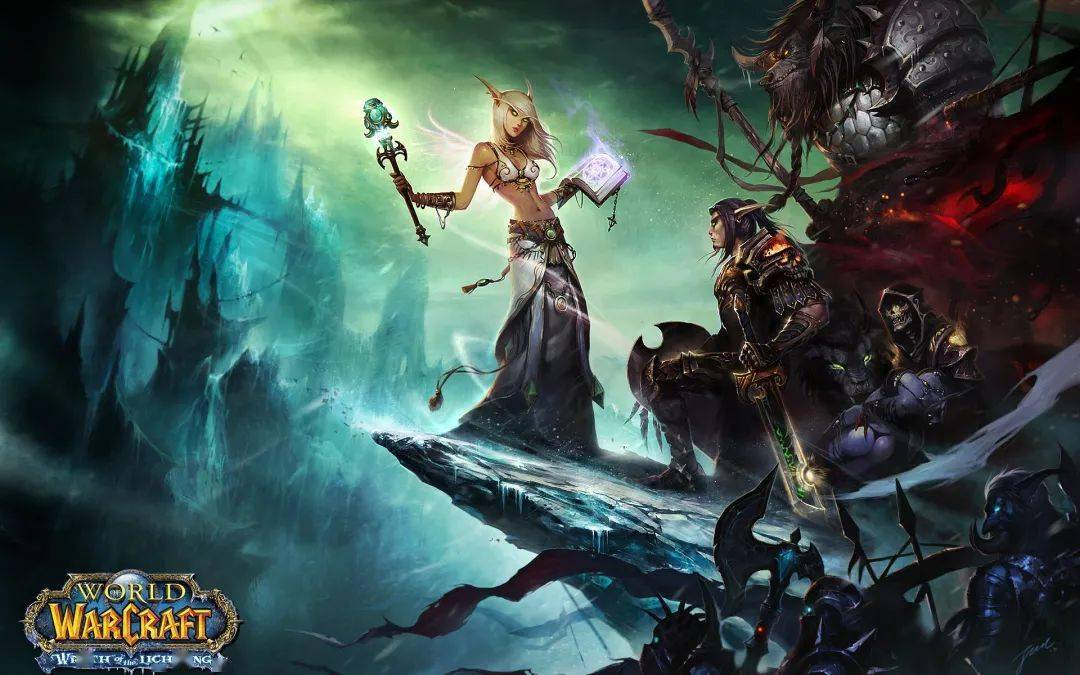
\includegraphics[width=0.8\textwidth]{figures/诺森德.jpg}
    \caption{诺森德远征}
    \label{fig:northrend}
\end{figure}